\chapter{第一章}

\section{公式的书写}

\begin{equation}
\label{eq-1}
    \mathbf{A} = \mathbf{B} \mathbf{C}^T
\end{equation}

\section{图的绘制}

\begin{figure}
    \vspace{1em}
    \centering
    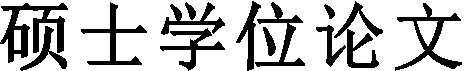
\includegraphics[width=0.7\linewidth]{figures/master-hwzs.pdf}
    \bicaption[fig:example]{示例图片}{示例图片}{Fig.}{Example}
\end{figure}

\section{三线表的绘制}

\begin{table}[h]
    \bicaption[tab:example]{三线表示例}{三线表示例\vspace{-0.3cm}}{Tab.}{Table example}
    \centering
    \vspace{0.2cm}
    \wuhao
    \begin{tabular}{cc}
        \hline
        列1 & 列2  \\
        \hline
        数据1 & 数据2 \\
        数据3 & 数据4 \\
        \hline
    \end{tabular}
\end{table}

\section{算法流程的书写}

\begin{figure}
    \centering
    \begin{minipage}{0.75\linewidth}
        \begin{algorithm}[H]
            \caption{示例算法}
            \label{alg-1}
            \begin{algorithmic}[1]
                \Require 原始数据 $\mathbf{X}$
                \Ensure 结果 $\mathbf{Y}$
                \State 普通语句;
                \For{$i = 1 : n$}
                    \State 循环逻辑;
                \EndFor
            \end{algorithmic}
        \end{algorithm}
    \end{minipage}
\end{figure}

\section{列表的使用}

\begin{asparaenum}[(1)]
    \item 第一项;
    \item 第二项。
\end{asparaenum}


% 清除空白页
\let\cleardoublepage\clearpage



